\documentclass[11pt,a4paper]{article}

\usepackage[ngerman]{babel}
\usepackage[TS1,T1]{fontenc}
\usepackage[utf8x]{inputenc}
\usepackage{theorem}
\usepackage[scaled=0.9]{helvet}
\usepackage{amsmath}
\usepackage{amssymb}
\usepackage[T1]{fontenc}
\usepackage{hyperref}
\usepackage{stmaryrd}
\usepackage{pgf,tikz}
\usepackage{relsize}
\usepackage{enumitem}
\usepackage{graphicx}
\usepackage{algpseudocode,amsmath,xifthen}

\newcounter{numb}
\theoremstyle{break}
\theorembodyfont{\upshape}
   	\newtheorem{aufgabe}{Aufgabe}[numb]
\setcounter{numb}{2}
\setlength{\oddsidemargin}{0cm}
\setlength{\textwidth}{16cm}
\setlength{\textheight}{23cm}
\setlength{\topmargin}{-2cm}

\usetikzlibrary{shapes,arrows,automata,positioning,decorations.fractals}
\renewcommand\familydefault{\sfdefault}


\begin{document}

\begin{minipage}[b]{\textwidth}
\parbox[t]{5cm}{%

\includegraphics[width=4cm]{unilogo}
\hfill
}
\parbox[b]{11cm}{%
%\scshape%
Heinrich-Heine-Universit\"at D\"usseldorf\\
Institut f\"ur Informatik\\
Lehrstuhl Softwaretechnik und Programmiersprachen\\
%Professor Dr.\ M.\ Leuschel
Philipp K\"orner
}

%%date
%\hfill 1.\@ August 2017\rule{0mm}{6mm}\quad\ %% <--
\end{minipage}
\begin{center}
\bf
Funktionale Programmierung -- WS 2020 / 2021\\
Reading Guide 2: Datenstrukturen und Laziness
\end{center}

\pagestyle{empty}

\paragraph{Zeitliche Orientierung:} Diese Lerneinheit sollte bis zum 19.11.2020 abgeschlossen werden.
%\paragraph{Abgabe des Lerntagebuchs} \"uber das ILIAS bis zum 16.5.2020 mit unbegrenzt Material, Nachfrist bis zum 23.5.2020 mit zwei Seiten A4.

\section{Material} 

\begin{itemize}
\item Clojure for the Brave and True, Kapitel 4
\item The Joy of Clojure, Kapitel 6
\item Rich Hickey: Clojure for Java Programmers \url{https://www.youtube.com/watch?v=P76Vbsk_3J0} (ab 1:35:38)
\item Rich Hickey: Clojure for Java Programmers Part 2 \url{https://www.youtube.com/watch?v=hb3rurFxrZ8} (24:00 bis bis 29:06)
\item Rich Hickey: Persistent Data Structures and Managed References \url{https://www.infoq.com/presentations/Value-Identity-State-Rich-Hickey/} (17:20 bis 32:40)
\item 02\_data.clj
\item 04\_destructuring.clj
\item 05\_recursion.clj 
\item 09\_evaluation\_order.clj
\end{itemize}


\section{Lernziele}

Nach dem Bearbeiten dieser Lerneinheit sollten Sie in der Lage sein

\begin{itemize}
    \item die Implementierung von Listen, Vektoren, Sets und Maps in Clojure darzustellen.
    \item die Laufzeitcharakteristika von Listen, Vektoren, Sets und Maps bei verschiedenen Operationen zu benennen.
    \item Structural Sharing, Immutability und deren Zusammenhang zu erkl\"aren.
    \item die M\"oglichkeiten f\"ur Structural Sharing bei gegebenen Datenstrukturen und Operationen zu identifizieren.
    \item das Konzept von Laziness zu beschreiben.
    \item zu entscheiden, welche Berechnungen in Clojure direkt und welche verzögert ausgef\"uhrt werden (k\"onnen).
    \item zwischen impliziter und expliziter Laziness zu unterscheiden und den Unterschied zu erkl\"aren.
    \item Destrukturierung von Datenstrukturen zu lesen und die Bindung der Symbole anzugeben.
    \item selbst rekursive Programme zu implementieren.
\end{itemize}

\section{Highlights}

\begin{itemize}
    \item Immutability
    \item Structural Sharing
    \item Laziness
    \item Destrukturierung
    \item Auswertungsregeln, Scoping
    \item Implementierung des Hash Array-Mapped Trie (insb. Path Copying)
    \item Special Forms: \verb|loop|, \verb|recur|
    \item Funktionen: \verb|trampoline|, \verb|concat|, \verb|mapcat|, \verb|take|, \verb|drop|, \verb|nth|, \verb|count|, \verb|last|
\end{itemize}



\section{Aufgaben}
\begin{aufgabe}[Hash Trie]

    In dieser Aufgabe betrachten wir einen Hash Trie mit einem branching factor von 4,
    d.h. jeder Knoten hat maximal 4 Nachfolger.
    Nehmen Sie f\"ur diese Aufgabe die folgenden Hashwerte an:

    \begin{center}
    \begin{tabular}{l@{}ll@{}l}
        hash(:a)    &= \colorbox{red!15}{00}\colorbox{blue!15}{10}\colorbox{orange!15}{00}\colorbox{green!15}{00} &hash(:e)    &= \colorbox{red!15}{10}\colorbox{blue!15}{01}\colorbox{orange!15}{11}\colorbox{green!15}{01}\\
        hash(:b)    &= \colorbox{red!15}{10}\colorbox{blue!15}{00}\colorbox{orange!15}{00}\colorbox{green!15}{10} &hash(:new)  &= \colorbox{red!15}{00}\colorbox{blue!15}{01}\colorbox{orange!15}{01}\colorbox{green!15}{10}\\
        hash(:c)    &= \colorbox{red!15}{01}\colorbox{blue!15}{11}\colorbox{orange!15}{10}\colorbox{green!15}{10} &hash(:ouch) &= \colorbox{red!15}{11}\colorbox{blue!15}{01}\colorbox{orange!15}{11}\colorbox{green!15}{01}\\
        hash(:d)    &= \colorbox{red!15}{11}\colorbox{blue!15}{00}\colorbox{orange!15}{01}\colorbox{green!15}{00} &\\
    \end{tabular}
    \end{center}

\begin{center}
    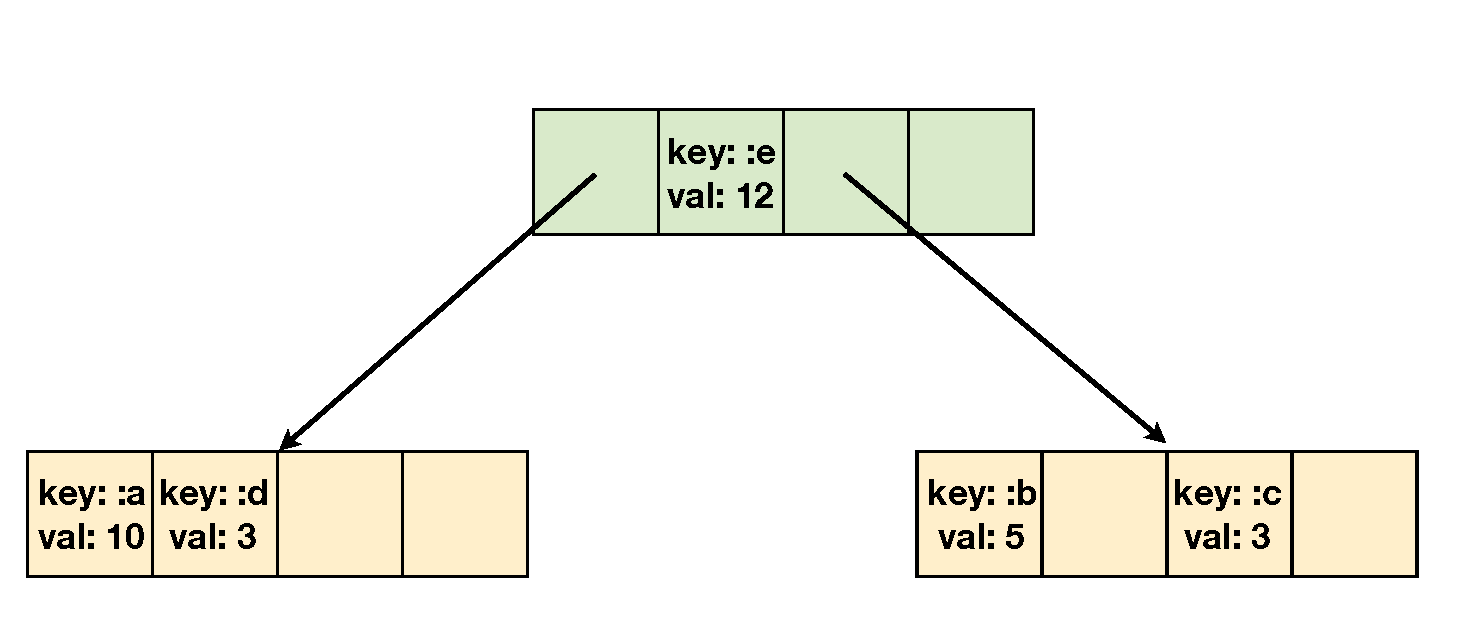
\includegraphics[scale=0.4]{hashtrie.pdf}
\end{center}

\begin{enumerate}[label=\alph*)]
\item
    Welche Map speichert der abgebildete Trie?
\item
    Wie viele Bits werden zur Bestimmung der Position in einem Array verwendet?
\item
    F\"ugen Sie unter dem Schl\"ussel \texttt{:new} den Wert \texttt{:ez} ein.
    Welche Knoten k\"onnen \"ubernommen werden, welche werden kopiert?
\item
    F\"ugen Sie unter dem Schl\"ussel \texttt{:ouch} den Wert \texttt{:almost-a-collision} ein.
    Welche Knoten k\"onnen \"ubernommen werden, welche werden kopiert?
\end{enumerate}
\end{aufgabe}


\pagebreak

\begin{aufgabe}[Maxima]

\begin{enumerate}[label=\alph*)]
\item
  Geben Sie eine Funktion an, die den maximalen Wert seiner Argumente bestimmt.
\begin{verbatim}
(max-value 3 42 1336 12.5)
=> 1336
\end{verbatim}
\item
  Geben Sie eine Funktion an, die die erste l\"angste Sequenz ihrer Argumente bestimmt. Verschachtelungen sollen hier nicht betrachtet werden.
\begin{verbatim}
(longest []  [:a :b 12] [[1 2 3 4 5 6]])
=> [:a :b 12]
\end{verbatim}
\item
  Geben Sie eine Funktion an, die die maximale L\"ange ihrer Argumente bestimmt. Verschachtelungen sollen auch hier nicht betrachtet werden.
\begin{verbatim}
(max-length []  [:a :b 12] [[1 2 3 4 5 6]])
=> 3
\end{verbatim}

\end{enumerate}
\end{aufgabe}



\begin{aufgabe}[Matrix]
Im Folgenden betrachen wir eine Matrix als Vektor von Zeilenvektoren. Zum Beispiel:
\begin{verbatim}
(def einheitsmatrix [[1 0 0] [0 1 0] [0 0 1]])
(def matrix2 [[1 0 0 1] [0 1 0 1] [0 0 1 1]])
\end{verbatim}

\begin{enumerate}[label=\alph*)]
\item Schreiben Sie eine Funktion p!, die eine Matrix ausgibt. 
\begin{verbatim}
user=> (p! einheitsmatrix)
100
010
001
\end{verbatim}
  
\item Schreiben Sie eine Funktion trans, die die Matrix transponiert, d.h., Zeilen und Spalten vertauscht:
\begin{verbatim}
user=> (= einheitsmatrix (trans einheitsmatrix))
true
user=> (p! (trans matrix2))
100
010
001
111
user=> (= matrix2 (trans matrix2))
false
user=> (= matrix2 (trans (trans matrix2)))
true 
\end{verbatim}
\end{enumerate}

\end{aufgabe}

\begin{aufgabe}[Black Box Testing (4clojure \#65)]
    Clojure hat verschiedene Collections, die sich aber (leicht) im Verhalten unterscheiden.
    Die Funktionen aus \verb|clojure.core| wandeln diese typischerweise in Sequenzen um und arbeiten darauf.
    Es ist aber wichtig, das Verhalten und die Performanceunterschiede genau zu verstehen,
    um zu entscheiden, welche Repr\"asentation von Daten angemessen ist.

    Schreiben Sie eine Funktion \verb|data-type|, die eine Collection als Parameter nimmt und \verb|:map|, \verb|:set|, \verb|:list| oder \verb|:vector| zur\"uckgibt,
    je nach dem welche Art Collection eingegeben wird.

    Es ist nicht erlaubt, Pr\"adikate wie \verb|list?| zu verwenden.
    Die Aufgabe ist es, mit den Collections zu spielen und das Verhalten zu verstehen.
\end{aufgabe}

\section*{Fragen}
Bei Fragen wenden Sie sich bitte an Philipp K"orner (\texttt{p.koerner@hhu.de}).
\end{document}

